\documentclass[11pt,a4paper]{article}

\usepackage[utf8]{inputenc}
\usepackage[T1]{fontenc}
\usepackage{mathpazo}
\usepackage[scaled=0.92]{helvet}
\usepackage[margin=1in]{geometry}
\usepackage{graphicx}
\usepackage{amsmath,amssymb,amsfonts}
\usepackage{booktabs}
\usepackage{tabularx}
\usepackage{setspace}
\usepackage{titlesec}
\usepackage{fancyhdr}
\usepackage{float}
\usepackage{caption}
\usepackage{microtype}

\usepackage{tikz}
\usetikzlibrary{shapes.geometric, arrows.meta, positioning, calc, matrix, fit, backgrounds}

\usepackage{listings}
\usepackage{xcolor}
\usepackage[hidelinks]{hyperref}

\setstretch{1.15}
\setlength{\parindent}{0pt}
\setlength{\parskip}{0.8em}
\sloppy

\titleformat{\section}{\normalfont\large\bfseries\sffamily}{\thesection}{1em}{}
\titleformat{\subsection}{\normalfont\normalsize\bfseries\sffamily}{\thesubsection}{1em}{}
\titleformat{\subsubsection}{\normalfont\normalsize\itshape\sffamily}{\thesubsubsection}{1em}{}

\pagestyle{fancy}
\fancyhf{}
\fancyhead[L]{\small\sffamily Fondasi Basis Data: CRUD pada Tingkat Tabel}
\fancyhead[R]{\small\sffamily\thepage}
\renewcommand{\headrulewidth}{0.4pt}

\captionsetup{font=small,labelfont=bf,labelsep=period}

\renewenvironment{abstract}
{\small
	\begin{center}\textbf{\sffamily Abstrak}\end{center}
	\begin{quote}}
	{\end{quote}}

\lstdefinestyle{code}{
	basicstyle=\ttfamily\small,
	frame=single,
	rulecolor=\color{black},
	breaklines=true,
	showstringspaces=false,
	columns=fullflexible,
	keepspaces=true,
	framesep=6pt,
	aboveskip=1em,
	belowskip=1em,
	xleftmargin=0pt
}

\lstdefinestyle{out}{
	basicstyle=\ttfamily\small,
	frame=tb,
	rulecolor=\color{black},
	breaklines=true,
	showstringspaces=false,
	columns=fullflexible,
	keepspaces=true,
	framesep=4pt,
	aboveskip=1em,
	belowskip=1em
}

\title{\vspace{-1.5cm}\textbf{\sffamily\LARGE Fondasi Basis Data: Menguasai CRUD pada Tingkat Tabel}}
\author{
	\textbf{Muhammad Riduwan Khafidi} \\
	\small Program Studi Teknik Rekayasa Perangkat Lunak \\
	\small Politeknik Negeri Batam \\
	\small \texttt{4342611034@students.polibatam.ac.id}
}
\date{\small\today}

\begin{document}

\maketitle
\thispagestyle{empty}

\begin{abstract}
	Tabel adalah unit struktural terkecil yang utuh di dalam basis data relasional. Setelah database dibuat, seluruh pekerjaan berikutnya berkutat pada tabel: mendefinisikan kolom, menetapkan batasan, menambahkan indeks, mengubah struktur saat kebutuhan berubah, dan pada akhirnya menghapus tabel yang sudah tidak terpakai. Makalah ini membahas CRUD pada tingkat tabel secara menyeluruh, mulai dari \texttt{CREATE TABLE} dengan seluruh klausa batasannya, \texttt{SHOW TABLES} dan \texttt{DESCRIBE} sebagai jendela pengamatan struktur, \texttt{ALTER TABLE} dengan dua belas varian operasinya, hingga \texttt{DROP TABLE} dan \texttt{TRUNCATE TABLE} beserta perbedaan konsekuensinya. Setiap perintah dilengkapi diagram anatomi, simulasi keluaran, dan skenario yang lazim dijumpai di dunia kerja. Makalah ini melanjutkan makalah CRUD Database dan menjadi fondasi sebelum pembaca melangkah ke CRUD pada tingkat baris.
\end{abstract}

\section{Pendahuluan: Tabel sebagai Unit Struktural}

\subsection{Analogi Lemari Arsip}

Database adalah ruangan. Tabel adalah lemari arsip di dalamnya. Setiap lemari punya laci-laci bernomor, dan setiap laci diberi label yang jelas: nomor, nama, tanggal, isi. Sebelum kertas dimasukkan ke dalam laci, lemarinya harus dibangun dulu, lacinya ditentukan jumlahnya, dan labelnya dipasang.

Dalam basis data, membangun lemari itu disebut \texttt{CREATE TABLE}. Menentukan jumlah dan nama laci disebut mendefinisikan kolom. Memberi aturan bahwa laci nomor tidak boleh kosong disebut \texttt{NOT NULL}. Memberi aturan bahwa satu nomor hanya boleh muncul sekali disebut \texttt{PRIMARY KEY}. Semua itu terjadi sebelum satu baris data pun masuk.

\subsection{Batas antara Struktur dan Isi}

Penting membedakan dua hal yang sering tertukar:

\begin{itemize}
	\item Struktur tabel: kolom apa saja yang ada, tipe datanya apa, batasannya apa, indeksnya apa. Ini wilayah \texttt{CREATE}, \texttt{ALTER}, dan \texttt{DROP}.
	\item Isi tabel: baris-baris data yang tersimpan. Ini wilayah \texttt{INSERT}, \texttt{SELECT}, \texttt{UPDATE}, dan \texttt{DELETE}.
\end{itemize}

Makalah ini fokus pada struktur. Isi akan dibahas di makalah berikutnya. Namun keduanya bertemu di satu titik: \texttt{TRUNCATE TABLE} menghapus seluruh isi tetapi mempertahankan struktur, sedangkan \texttt{DROP TABLE} menghapus keduanya sekaligus.

\subsection{Siklus Hidup CRUD Tabel}

Gambar~\ref{fig:crud-cycle} merangkum empat operasi yang akan dibahas sepanjang makalah ini.

\begin{figure}[H]
	\centering
	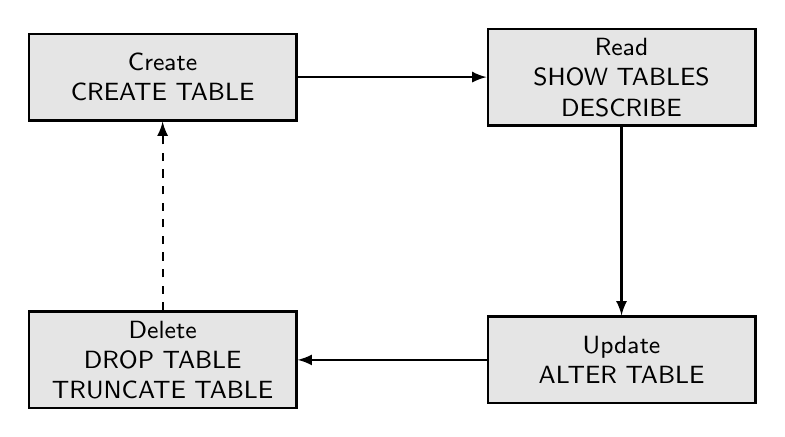
\begin{tikzpicture}[
			node distance=2.4cm,
			op/.style={rectangle, draw=black, thick, fill=black!10, minimum width=3.4cm, minimum height=1.1cm, align=center, font=\sffamily\small},
			cmd/.style={font=\ttfamily\scriptsize},
			line/.style={draw, thick, -latex}
		]
		\node[op] (create) {Create \\ \cmd{CREATE TABLE}};
		\node[op, right=of create] (read) {Read \\ \cmd{SHOW TABLES} \\ \cmd{DESCRIBE}};
		\node[op, below=of read] (update) {Update \\ \cmd{ALTER TABLE}};
		\node[op, left=of update] (delete) {Delete \\ \cmd{DROP TABLE} \\ \cmd{TRUNCATE TABLE}};

		\draw[line] (create) -- (read);
		\draw[line] (read) -- (update);
		\draw[line] (update) -- (delete);
		\draw[line, dashed] (delete) -- (create);
	\end{tikzpicture}
	\caption{Siklus hidup CRUD pada tingkat tabel.}
	\label{fig:crud-cycle}
\end{figure}

Garis putus-putus dari \texttt{DROP} kembali ke \texttt{CREATE} menandakan skenario umum di dunia kerja: struktur tabel berubah drastis sehingga lebih mudah menghapus dan membuat ulang daripada meng-ubah satu per satu.

\section{Konteks: Berada di Dalam Database}

Sebelum semua perintah tabel bisa dijalankan, kita harus berada di dalam sebuah database. Ini berbeda dengan perintah database yang bisa dijalankan dari mana saja.

\begin{lstlisting}[style=code]
USE toko_online;
SELECT DATABASE();
\end{lstlisting}

\begin{lstlisting}[style=out]
+--------------+
| DATABASE()   |
+--------------+
| toko_online  |
+--------------+
\end{lstlisting}

Jika \texttt{SELECT DATABASE()} mengembalikan \texttt{NULL}, artinya belum ada database yang dipilih, dan perintah tabel akan gagal dengan pesan \texttt{No database selected}.

\section{Create: Mendirikan Tabel}

\subsection{Sintaks Dasar}

Bentuk minimal \texttt{CREATE TABLE} membutuhkan setidaknya satu kolom. Tanpa kolom, MariaDB menolak.

\begin{lstlisting}[style=code]
CREATE TABLE nama_tabel (
    nama_kolom1 tipe_data [batasan],
    nama_kolom2 tipe_data [batasan],
    ...
    [batasan tingkat tabel]
);
\end{lstlisting}

Jika dicoba tanpa kolom, hasilnya seperti ini.

\begin{lstlisting}[style=code]
CREATE TABLE kosong;
\end{lstlisting}

\begin{lstlisting}[style=out]
ERROR 1113 (42000): A table must have at least 1 column
\end{lstlisting}

\subsection{Anatomi Satu Kolom}

Setiap kolom terdiri dari tiga bagian: nama, tipe data, dan batasan opsional. Gambar~\ref{fig:anatomy} memvisualkan anatomi tersebut pada satu tabel contoh.

\begin{figure}[H]
	\centering
	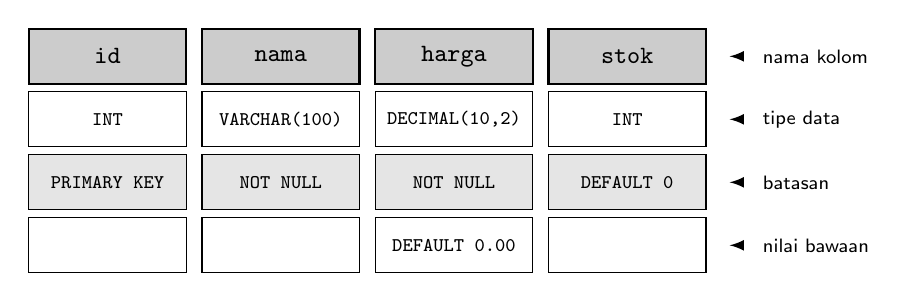
\begin{tikzpicture}[
			hdr/.style={rectangle, draw=black, thick, fill=black!20, minimum width=2cm, minimum height=0.7cm, font=\ttfamily\small, align=center},
			cell/.style={rectangle, draw=black, minimum width=2cm, minimum height=0.7cm, font=\ttfamily\scriptsize, align=center},
			note/.style={font=\scriptsize\sffamily, align=left},
			arr/.style={draw, thick, -latex}
		]
		\node[hdr] (h1) at (0,3) {id};
		\node[hdr] (h2) at (2.2,3) {nama};
		\node[hdr] (h3) at (4.4,3) {harga};
		\node[hdr] (h4) at (6.6,3) {stok};

		\node[cell] (c1) at (0,2.2) {INT};
		\node[cell] (c2) at (2.2,2.2) {VARCHAR(100)};
		\node[cell] (c3) at (4.4,2.2) {DECIMAL(10,2)};
		\node[cell] (c4) at (6.6,2.2) {INT};

		\node[cell, fill=black!10] (k1) at (0,1.4) {PRIMARY KEY};
		\node[cell, fill=black!10] (k2) at (2.2,1.4) {NOT NULL};
		\node[cell, fill=black!10] (k3) at (4.4,1.4) {NOT NULL};
		\node[cell, fill=black!10] (k4) at (6.6,1.4) {DEFAULT 0};

		\node[cell, fill=white] (d3) at (4.4,0.6) {DEFAULT 0.00};
		\node[cell, fill=white] (d1) at (0,0.6) {\ };
		\node[cell, fill=white] (d2) at (2.2,0.6) {\ };
		\node[cell, fill=white] (d4) at (6.6,0.6) {\ };

		\node[note, anchor=west] at (8.2, 3) {nama kolom};
		\node[note, anchor=west] at (8.2, 2.2) {tipe data};
		\node[note, anchor=west] at (8.2, 1.4) {batasan};
		\node[note, anchor=west] at (8.2, 0.6) {nilai bawaan};

		\draw[arr] (8.0,3) -- (7.9,3);
		\draw[arr] (8.0,2.2) -- (7.9,2.2);
		\draw[arr] (8.0,1.4) -- (7.9,1.4);
		\draw[arr] (8.0,0.6) -- (7.9,0.6);
	\end{tikzpicture}
	\caption{Anatomi kolom pada sebuah tabel.}
	\label{fig:anatomy}
\end{figure}

Bagian atas adalah nama kolom yang dipakai untuk merujuk kolom di query. Bagian tengah adalah tipe data yang sudah dibahas mendalam pada makalah sebelumnya. Bagian bawah adalah batasan yang menentukan aturan main kolom itu.

\subsection{Batasan (Constraint) yang Perlu Dikuasai}

MariaDB mendukung beberapa batasan utama di tingkat kolom dan tabel. Tabel~\ref{tab:constraints} merangkumnya.

\begin{table}[H]
	\centering
	\caption{Batasan (constraint) pada tabel MariaDB.}
	\label{tab:constraints}
	\small
	\begin{tabularx}{\textwidth}{l l X}
		\toprule
		Batasan                  & Tingkat          & Fungsi                            \\
		\midrule
		\texttt{NOT NULL}        & kolom            & kolom tidak boleh kosong          \\
		\texttt{DEFAULT}         & kolom            & nilai bawaan jika tidak diisi     \\
		\texttt{PRIMARY KEY}     & kolom atau tabel & kunci unik dan tidak boleh kosong \\
		\texttt{UNIQUE}          & kolom atau tabel & nilai harus unik, boleh kosong    \\
		\texttt{CHECK}           & kolom atau tabel & nilai harus memenuhi kondisi      \\
		\texttt{AUTO\_INCREMENT} & kolom            & isi otomatis dengan angka naik    \\
		\texttt{FOREIGN KEY}     & tabel            & merujuk ke primary key tabel lain \\
		\texttt{REFERENCES}      & kolom            & bagian dari sintaks foreign key   \\
		\bottomrule
	\end{tabularx}
\end{table}

Batasan di tingkat kolom ditulis langsung setelah tipe data. Batasan di tingkat tabel ditulis sebagai klausa tersendiri di akhir definisi, dan bisa merujuk lebih dari satu kolom. Contoh batasan tingkat tabel adalah \texttt{PRIMARY KEY (a, b)} untuk composite primary key.

\subsection{Varian \texttt{CREATE TABLE}}

MariaDB menyediakan beberapa varian yang berguna di skenario berbeda. Tabel~\ref{tab:create-variants} merangkumnya.

\begin{table}[H]
	\centering
	\caption{Varian \texttt{CREATE TABLE}.}
	\label{tab:create-variants}
	\small
	\begin{tabularx}{\textwidth}{l X}
		\toprule
		Varian                               & Kegunaan                                    \\
		\midrule
		\texttt{CREATE TABLE nama (...)}     & membuat tabel baru dari nol                 \\
		\texttt{CREATE TABLE IF NOT EXISTS}  & aman untuk skrip berulang                   \\
		\texttt{CREATE TEMPORARY TABLE}      & tabel sementara, hilang saat sesi ditutup   \\
		\texttt{CREATE TABLE baru LIKE lama} & menyalin struktur tanpa data                \\
		\texttt{CREATE TABLE baru AS SELECT} & menyalin struktur dan data dari hasil query \\
		\bottomrule
	\end{tabularx}
\end{table}

Varian \texttt{LIKE} sangat berguna untuk mengkloning tabel di lingkungan pengujian. Varian \texttt{AS SELECT} dipakai untuk membuat tabel laporan atau tabel ringkasan dari tabel sumber.

\subsection{Contoh Lengkap}

Berikut adalah perintah \texttt{CREATE TABLE} yang mendirikan tabel \texttt{produk} dengan tujuh kolom, masing-masing dengan alasan pemilihan tipe dan batasannya.

\begin{lstlisting}[style=code]
CREATE TABLE produk (
    id          BIGINT UNSIGNED  DEFAULT (UUID_SHORT()) PRIMARY KEY,
    nama        VARCHAR(150)     NOT NULL,
    harga       DECIMAL(12,2)    NOT NULL DEFAULT 0.00,
    stok        INT UNSIGNED     NOT NULL DEFAULT 0,
    deskripsi   TEXT,
    is_active   BOOLEAN          NOT NULL DEFAULT TRUE,
    created_at  DATETIME         DEFAULT CURRENT_TIMESTAMP
) COMMENT='Katalog produk toko online';
\end{lstlisting}

Keluaran jika berhasil.

\begin{lstlisting}[style=out]
Query OK, 0 rows affected
\end{lstlisting}

Kalimat \texttt{0 rows affected} konsisten dengan sifat operasi DDL (Data Definition Language) yang tidak menyentuh baris data. Angka nol itu mengacu pada baris, bukan pada tabel yang baru saja dibuat.

\subsection{Penjelasan Setiap Kolom}

\begin{itemize}
	\item \texttt{id BIGINT UNSIGNED DEFAULT (UUID\_SHORT()) PRIMARY KEY}: kunci utama 8 byte dengan nilai yang selalu bertambah secara monotonik, menghindari fragmentasi indeks.
	\item \texttt{nama VARCHAR(150) NOT NULL}: nama produk wajib diisi, panjang bervariasi, dibatasi 150 karakter agar indeks tetap ringan.
	\item \texttt{harga DECIMAL(12,2) NOT NULL DEFAULT 0.00}: uang wajib exact numeric, presisi 12 digit, 2 desimal.
	\item \texttt{stok INT UNSIGNED NOT NULL DEFAULT 0}: jumlah barang dalam stok, tidak boleh negatif, diisi nol secara bawaan.
	\item \texttt{deskripsi TEXT}: deskripsi panjang yang boleh kosong.
	\item \texttt{is\_active BOOLEAN NOT NULL DEFAULT TRUE}: penanda aktif atau tidak, otomatis aktif saat dibuat.
	\item \texttt{created\_at DATETIME DEFAULT CURRENT\_TIMESTAMP}: waktu pembuatan baris, otomatis terisi.
\end{itemize}

Perhatikan bahwa semua kolom yang wajib diisi diberi \texttt{NOT NULL}, dan semua kolom yang punya nilai wajar diberi \texttt{DEFAULT}. Hasilnya, \texttt{INSERT} hanya perlu menyebut kolom yang benar-benar esensial.

\subsection{Alur Keputusan Sebelum \texttt{CREATE TABLE}}

Gambar~\ref{fig:create-flow} menyajikan alur singkat sebelum mengeksekusi \texttt{CREATE TABLE}.

\begin{figure}[H]
	\centering
	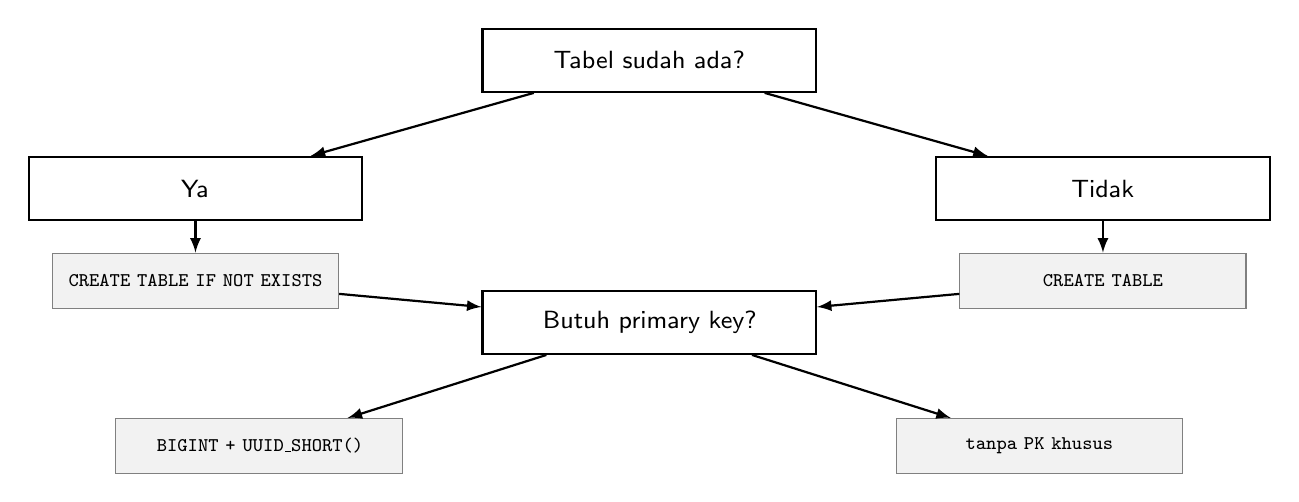
\begin{tikzpicture}[
			node distance=0.5cm and 1cm,
			q/.style={rectangle, draw=black, thick, fill=white, text width=4cm, align=center, minimum height=0.8cm, font=\sffamily\small},
			a/.style={rectangle, draw=black!50, fill=black!5, text width=3.4cm, align=center, minimum height=0.7cm, font=\ttfamily\scriptsize},
			line/.style={draw, thick, -latex}
		]
		\node[q] (start) {Tabel sudah ada?};
		\node[q, below left=0.8cm and 1.5cm of start] (yes) {Ya};
		\node[q, below right=0.8cm and 1.5cm of start] (no) {Tidak};
		\node[a, below=0.4cm of yes] (y1) {\texttt{CREATE TABLE IF NOT EXISTS}};
		\node[a, below=0.4cm of no] (n1) {\texttt{CREATE TABLE}};

		\node[q, below=2.5cm of start] (pk) {Butuh primary key?};
		\node[a, below left=0.8cm and 1cm of pk] (p1) {\texttt{BIGINT} + \texttt{UUID\_SHORT()}};
		\node[a, below right=0.8cm and 1cm of pk] (p2) {tanpa PK khusus};

		\draw[line] (start) -- (yes);
		\draw[line] (start) -- (no);
		\draw[line] (yes) -- (y1);
		\draw[line] (no) -- (n1);
		\draw[line] (y1) -- (pk);
		\draw[line] (n1) -- (pk);
		\draw[line] (pk) -- (p1);
		\draw[line] (pk) -- (p2);
	\end{tikzpicture}
	\caption{Alur keputusan sebelum \texttt{CREATE TABLE}.}
	\label{fig:create-flow}
\end{figure}

\section{Read: Mengintip Struktur Tabel}

Operasi Read pada tingkat tabel tidak menampilkan isi baris (itu \texttt{SELECT}), melainkan menampilkan struktur. Ada empat perintah yang bekerja sama untuk tujuan ini, masing-masing dengan tingkat kedalaman yang berbeda.

\subsection{Melihat Daftar Tabel}

\begin{lstlisting}[style=code]
SHOW TABLES;
\end{lstlisting}

\begin{lstlisting}[style=out]
+-----------------------+
| Tables_in_toko_online |
+-----------------------+
| pelanggan             |
| pesanan               |
| produk                |
+-----------------------+
3 rows in set (0.001 sec)
\end{lstlisting}

Untuk menyaring berdasarkan pola, gunakan \texttt{LIKE}.

\begin{lstlisting}[style=code]
SHOW TABLES LIKE 'prod%';
\end{lstlisting}

\subsection{Melihat Kolom dengan \texttt{DESCRIBE}}

\begin{lstlisting}[style=code]
DESCRIBE produk;
\end{lstlisting}

\begin{lstlisting}[style=out]
+-------------+-----------------+------+-----+------------------+
| Field       | Type            | Null | Key | Default          |
+-------------+-----------------+------+-----+------------------+
| id          | bigint unsigned | NO   | PRI | NULL             |
| nama        | varchar(150)    | NO   |     | NULL             |
| harga       | decimal(12,2)   | NO   |     | 0.00             |
| stok        | int unsigned    | NO   |     | 0                |
| deskripsi   | text            | YES  |     | NULL             |
| is_active   | tinyint(1)      | NO   |     | 1                |
| created_at  | datetime        | YES  |     | current_timestamp|
+-------------+-----------------+------+-----+------------------+
7 rows in set (0.002 sec)
\end{lstlisting}

Perhatikan bahwa \texttt{BOOLEAN} muncul sebagai \texttt{tinyint(1)}. Ini mengonfirmasi bahwa \texttt{BOOLEAN} hanyalah alias, bukan tipe tersendiri. Kolom \texttt{Key} menampilkan \texttt{PRI} untuk primary key, \texttt{UNI} untuk unique, dan \texttt{MUL} untuk indeks biasa.

Singkatan \texttt{DESC} bisa dipakai sebagai alternatif.

\begin{lstlisting}[style=code]
DESC produk;
SHOW COLUMNS FROM produk;
\end{lstlisting}

Ketiga perintah menghasilkan keluaran yang sama.

\subsection{Melihat Definisi Lengkap dengan \texttt{SHOW CREATE TABLE}}

Jika \texttt{DESCRIBE} hanya menampilkan ringkasan, \texttt{SHOW CREATE TABLE} menampilkan perintah \texttt{CREATE TABLE} yang akan dijalankan untuk membangun tabel persis seperti sekarang.

\begin{lstlisting}[style=code]
SHOW CREATE TABLE produk\G
\end{lstlisting}

\begin{lstlisting}[style=out]
*************************** 1. row ***************************
       Table: produk
Create Table: CREATE TABLE `produk` (
  `id` bigint(20) unsigned NOT NULL DEFAULT uuid_short(),
  `nama` varchar(150) NOT NULL,
  `harga` decimal(12,2) NOT NULL DEFAULT 0.00,
  `stok` int(10) unsigned NOT NULL DEFAULT 0,
  `deskripsi` text DEFAULT NULL,
  `is_active` tinyint(1) NOT NULL DEFAULT 1,
  `created_at` datetime DEFAULT current_timestamp(),
  PRIMARY KEY (`id`)
) ENGINE=InnoDB DEFAULT CHARSET=utf8mb4
  COLLATE=utf8mb4_unicode_ci
  COMMENT='Katalog produk toko online'
\end{lstlisting}

Perhatikan tulisan \texttt{\textbackslash G} di akhir perintah. Ini mengganti titik koma dan membuat keluaran ditampilkan secara vertikal, jauh lebih mudah dibaca untuk tabel lebar.

Keluaran \texttt{SHOW CREATE TABLE} menampilkan beberapa informasi tambahan yang tidak muncul di \texttt{DESCRIBE}, yaitu \texttt{ENGINE}, \texttt{CHARSET}, \texttt{COLLATE}, dan \texttt{COMMENT}.

\subsection{Melihat Indeks dengan \texttt{SHOW INDEX}}

\begin{lstlisting}[style=code]
SHOW INDEX FROM produk;
\end{lstlisting}

\begin{lstlisting}[style=out]
+--------+------------+----------+--------------+-------------+
| Table  | Non_unique | Key_name | Seq_in_index | Column_name |
+--------+------------+----------+--------------+-------------+
| produk |          0 | PRIMARY  |            1 | id          |
+--------+------------+----------+--------------+-------------+
1 row in set
\end{lstlisting}

Kolom \texttt{Non\_unique} bernilai \texttt{0} menandakan indeks unik. Primary key selalu unik. Indeks biasa akan bernilai \texttt{1}.

\subsection{Menelusuri Katalog dengan \texttt{information\_schema}}

Untuk kebutuhan otomatisasi, hasil \texttt{SHOW} bisa diperoleh lewat query SQL ke \texttt{information\_schema}, yang merupakan katalog metadata server.

\begin{lstlisting}[style=code]
SELECT table_name, engine, table_rows,
       data_length, index_length
FROM information_schema.tables
WHERE table_schema = 'toko_online';
\end{lstlisting}

\begin{lstlisting}[style=out]
+------------+--------+------------+-------------+--------------+
| table_name | engine | table_rows | data_length | index_length |
+------------+--------+------------+-------------+--------------+
| pelanggan  | InnoDB |         14 |       16384 |        16384 |
| pesanan    | InnoDB |         52 |       32768 |        16384 |
| produk     | InnoDB |          8 |       16384 |        16384 |
+------------+--------+------------+-------------+--------------+
\end{lstlisting}

Perintah \texttt{SHOW} cocok untuk dipakai secara manual di terminal. Query \texttt{information\_schema} cocok untuk dipakai di dalam aplikasi karena hasilnya bisa difilter, diurutkan, dan digabung dengan query lain.

\subsection{Perbandingan Empat Cara Melihat Struktur}

Gambar~\ref{fig:read-paths} merangkum kapan sebaiknya memakai perintah yang mana.

\begin{figure}[H]
	\centering
	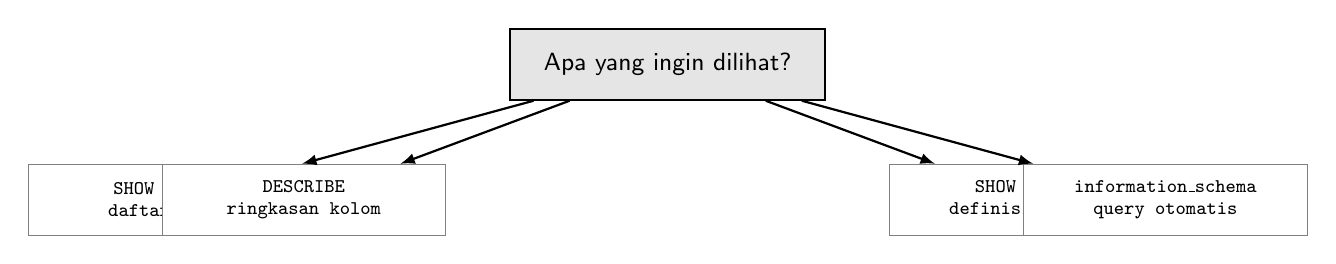
\begin{tikzpicture}[
			q/.style={rectangle, draw=black, thick, fill=black!10, minimum width=4cm, minimum height=0.9cm, align=center, font=\sffamily\small},
			a/.style={rectangle, draw=black!50, fill=white, minimum width=3.6cm, minimum height=0.9cm, align=center, font=\ttfamily\scriptsize},
			line/.style={draw, thick, -latex}
		]
		\node[q] (root) {Apa yang ingin dilihat?};

		\node[a, below left=0.8cm and 2.5cm of root] (tables) {\texttt{SHOW TABLES} \\ daftar tabel};
		\node[a, below left=0.8cm and 0.8cm of root] (cols) {\texttt{DESCRIBE} \\ ringkasan kolom};
		\node[a, below right=0.8cm and 0.8cm of root] (full) {\texttt{SHOW CREATE} \\ definisi lengkap};
		\node[a, below right=0.8cm and 2.5cm of root] (info) {\texttt{information\_schema} \\ query otomatis};

		\draw[line] (root) -- (tables);
		\draw[line] (root) -- (cols);
		\draw[line] (root) -- (full);
		\draw[line] (root) -- (info);
	\end{tikzpicture}
	\caption{Empat jalur untuk melihat struktur tabel sesuai kebutuhan.}
	\label{fig:read-paths}
\end{figure}

\section{Update: Mengubah Struktur dengan \texttt{ALTER TABLE}}

Inilah bagian terpanjang dari CRUD tabel. \texttt{ALTER TABLE} memiliki lebih dari sepuluh varian operasi, dan satu perintah bisa menggabungkan beberapa operasi sekaligus. Semua contoh di bawah menggunakan tabel \texttt{produk} dari bagian sebelumnya.

\subsection{Kerangka Umum}

\begin{lstlisting}[style=code]
ALTER TABLE nama_tabel
    operasi_1,
    operasi_2,
    ...
    operasi_n;
\end{lstlisting}

Setiap operasi dipisahkan koma. MariaDB akan menjalankan semuanya dalam satu transaksi DDL, artinya jika salah satu gagal, seluruh perubahan dibatalkan.

\subsection{Menambah Kolom: \texttt{ADD COLUMN}}

\begin{lstlisting}[style=code]
ALTER TABLE produk
    ADD COLUMN berat_gram INT UNSIGNED DEFAULT 0;
\end{lstlisting}

Kolom baru otomatis ditempatkan di akhir. Untuk menempatkannya di posisi tertentu, gunakan \texttt{FIRST} atau \texttt{AFTER}.

\begin{lstlisting}[style=code]
ALTER TABLE produk
    ADD COLUMN sku VARCHAR(20) NOT NULL AFTER id;
ALTER TABLE produk
    ADD COLUMN catatan TEXT FIRST;
\end{lstlisting}

Gambar~\ref{fig:add-col} mengilustrasikan perubahan struktur sebelum dan sesudah \texttt{ADD COLUMN}.

\begin{figure}[H]
	\centering
	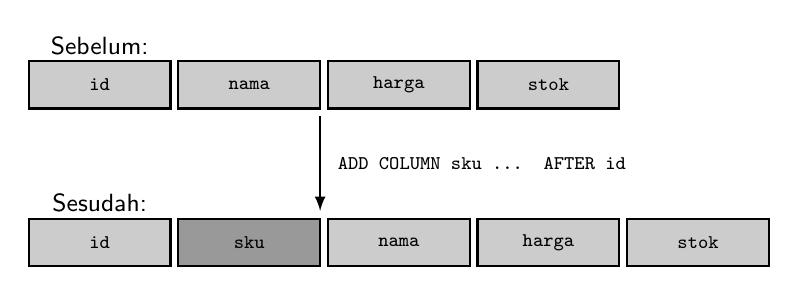
\begin{tikzpicture}[
			hdr/.style={rectangle, draw=black, thick, fill=black!20, minimum width=1.8cm, minimum height=0.6cm, font=\ttfamily\scriptsize, align=center},
			new/.style={rectangle, draw=black, thick, fill=black!40, minimum width=1.8cm, minimum height=0.6cm, font=\ttfamily\scriptsize, align=center},
			lbl/.style={font=\sffamily\small},
			arr/.style={draw, thick, -latex}
		]
		\node[lbl] at (0, 1.5) {Sebelum:};
		\node[hdr] (a1) at (0,1) {id};
		\node[hdr] (a2) at (1.9,1) {nama};
		\node[hdr] (a3) at (3.8,1) {harga};
		\node[hdr] (a4) at (5.7,1) {stok};

		\node[lbl] at (0, -0.5) {Sesudah:};
		\node[hdr] (b1) at (0,-1) {id};
		\node[new] (b2) at (1.9,-1) {sku};
		\node[hdr] (b3) at (3.8,-1) {nama};
		\node[hdr] (b4) at (5.7,-1) {harga};
		\node[hdr] (b5) at (7.6,-1) {stok};

		\draw[arr] (2.8, 0.6) -- (2.8, -0.6);
		\node[font=\scriptsize\sffamily, anchor=west] at (2.9, 0) {\texttt{ADD COLUMN sku ... AFTER id}};
	\end{tikzpicture}
	\caption{Efek \texttt{ADD COLUMN ... AFTER} pada struktur tabel.}
	\label{fig:add-col}
\end{figure}

\subsection{Menghapus Kolom: \texttt{DROP COLUMN}}

\begin{lstlisting}[style=code]
ALTER TABLE produk DROP COLUMN catatan;
\end{lstlisting}

Operasi ini menghapus kolom beserta seluruh datanya. Tidak ada undo. Jika kolom itu bagian dari indeks, indeks tersebut ikut terhapus atau perlu didefinisikan ulang. Jika kolom itu dirujuk oleh foreign key dari tabel lain, operasi akan ditolak.

\subsection{Mengubah Definisi Kolom: \texttt{MODIFY COLUMN}}

\texttt{MODIFY} mengubah tipe data, batasan, atau posisi kolom, tanpa mengubah namanya.

\begin{lstlisting}[style=code]
ALTER TABLE produk
    MODIFY COLUMN nama VARCHAR(200) NOT NULL;
\end{lstlisting}

Jika tipe data baru lebih kecil dan ada data yang tidak muat, MariaDB menolak operasi dengan pesan \texttt{Data truncated for column}. Jika tipe data baru lebih besar, operasi berhasil dan data lama tetap utuh.

\subsection{Mengubah Nama Kolom: \texttt{CHANGE COLUMN}}

\texttt{CHANGE} mengubah nama sekaligus definisi. Kedua hal harus disebutkan meskipun hanya salah satu yang berubah.

\begin{lstlisting}[style=code]
ALTER TABLE produk
    CHANGE COLUMN berat_gram berat INT UNSIGNED DEFAULT 0;
\end{lstlisting}

Perbedaan filosofis \texttt{MODIFY} dan \texttt{CHANGE} ditunjukkan pada Gambar~\ref{fig:modify-change}.

\begin{figure}[H]
	\centering
	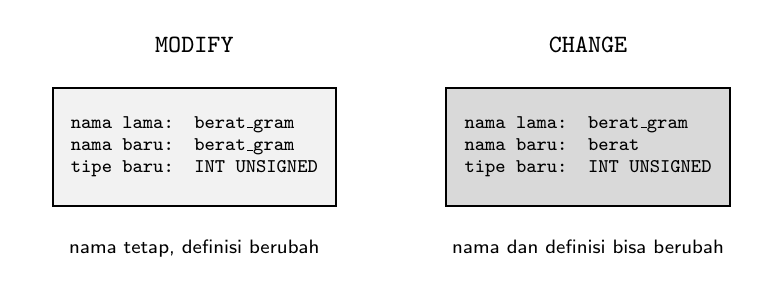
\begin{tikzpicture}[
			box/.style={rectangle, draw=black, thick, minimum width=3.6cm, minimum height=1.5cm, align=left, font=\ttfamily\scriptsize, inner sep=6pt},
			lbl/.style={font=\sffamily\small, align=center}
		]
		\node[lbl] (ml) at (-2.5, 1) {\texttt{MODIFY}};
		\node[box, fill=black!5] (mod) at (-2.5, -0.3) {
			nama lama: \texttt{berat\_gram} \\
			nama baru: \texttt{berat\_gram} \\
			tipe baru: \texttt{INT UNSIGNED}
		};
		\node[font=\scriptsize\sffamily, below=0.3cm of mod, text width=4cm, align=center] {nama tetap, definisi berubah};

		\node[lbl] (cl) at (2.5, 1) {\texttt{CHANGE}};
		\node[box, fill=black!15] (chg) at (2.5, -0.3) {
			nama lama: \texttt{berat\_gram} \\
			nama baru: \texttt{berat} \\
			tipe baru: \texttt{INT UNSIGNED}
		};
		\node[font=\scriptsize\sffamily, below=0.3cm of chg, text width=4cm, align=center] {nama dan definisi bisa berubah};
	\end{tikzpicture}
	\caption{Perbedaan \texttt{MODIFY COLUMN} dan \texttt{CHANGE COLUMN}.}
	\label{fig:modify-change}
\end{figure}

\subsection{Mengganti Nama Tabel: \texttt{RENAME TO}}

\begin{lstlisting}[style=code]
ALTER TABLE produk RENAME TO produk_lama;
ALTER TABLE produk_lama RENAME TO produk;
\end{lstlisting}

Operasi ini hanya mengganti nama, tidak menyentuh struktur maupun data. Berbeda dengan database yang tidak punya \texttt{RENAME}, tabel MariaDB mendukung \texttt{RENAME} secara langsung.

\subsection{Menambah dan Menghapus Indeks}

Indeks adalah struktur tambahan yang mempercepat pencarian pada kolom yang sering difilter.

\begin{lstlisting}[style=code]
ALTER TABLE produk
    ADD INDEX idx_harga (harga);
ALTER TABLE produk
    DROP INDEX idx_harga;
\end{lstlisting}

Untuk indeks unik, gunakan \texttt{ADD UNIQUE}.

\begin{lstlisting}[style=code]
ALTER TABLE produk
    ADD UNIQUE idx_sku (sku);
\end{lstlisting}

Gambar~\ref{fig:index-effect} menunjukkan mengapa indeks mempercepat pencarian.

\begin{figure}[H]
	\centering
	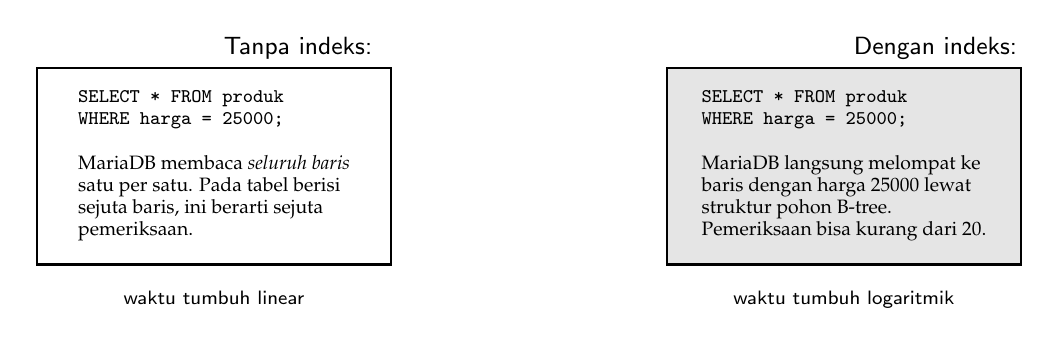
\begin{tikzpicture}[
			box/.style={rectangle, draw=black, thick, minimum width=4.5cm, minimum height=2.5cm, align=left, font=\scriptsize, inner sep=8pt},
			hdr/.style={font=\sffamily\small, anchor=west}
		]
		\node[hdr] at (-6, 1.5) {Tanpa indeks:};
		\node[box, fill=white] (noidx) at (-6, 0) {
			\texttt{SELECT * FROM produk} \\
			\texttt{WHERE harga = 25000;} \\
			\ \\
			MariaDB membaca \textit{seluruh baris} \\
			satu per satu. Pada tabel berisi \\
			sejuta baris, ini berarti sejuta \\
			pemeriksaan.
		};

		\node[hdr] at (2, 1.5) {Dengan indeks:};
		\node[box, fill=black!10] (idx) at (2, 0) {
			\texttt{SELECT * FROM produk} \\
			\texttt{WHERE harga = 25000;} \\
			\ \\
			MariaDB langsung melompat ke \\
			baris dengan harga 25000 lewat \\
			struktur pohon B-tree. \\
			Pemeriksaan bisa kurang dari 20.
		};

		\node[font=\scriptsize\sffamily, below=0.2cm of noidx, text width=4.5cm, align=center] {waktu tumbuh linear};
		\node[font=\scriptsize\sffamily, below=0.2cm of idx, text width=4.5cm, align=center] {waktu tumbuh logaritmik};
	\end{tikzpicture}
	\caption{Efek indeks pada kecepatan pencarian.}
	\label{fig:index-effect}
\end{figure}

\subsection{Menambah dan Menghapus Primary Key}

Tabel yang dibuat tanpa primary key bisa ditambahi setelahnya, asalkan kolomnya memenuhi syarat unik dan tidak ada nilai \texttt{NULL}.

\begin{lstlisting}[style=code]
ALTER TABLE produk ADD PRIMARY KEY (id);
ALTER TABLE produk DROP PRIMARY KEY;
\end{lstlisting}

Karena satu tabel hanya boleh punya satu primary key, \texttt{DROP PRIMARY KEY} selalu menghapus satu-satunya primary key yang ada. Jika kolomnya juga \texttt{AUTO\_INCREMENT}, operasi akan ditolak sampai \texttt{AUTO\_INCREMENT} dilepas lebih dulu.

\subsection{Menambah dan Menghapus Foreign Key}

\begin{lstlisting}[style=code]
ALTER TABLE pesanan
    ADD CONSTRAINT fk_pesanan_produk
        FOREIGN KEY (produk_id) REFERENCES produk(id);
ALTER TABLE pesanan DROP FOREIGN KEY fk_pesanan_produk;
\end{lstlisting}

Foreign key memaksa nilai \texttt{produk\_id} di tabel \texttt{pesanan} merujuk ke salah satu \texttt{id} yang ada di tabel \texttt{produk}. Ini menjaga integritas referensial, tetapi juga berarti bahwa \texttt{DROP TABLE produk} akan ditolak selama masih ada tabel lain yang merujuknya.

\subsection{Menggabungkan Beberapa Operasi}

Salah satu keunggulan \texttt{ALTER TABLE} adalah kemampuannya menggabungkan beberapa operasi dalam satu perintah, sehingga tabel hanya dibaca dan ditulis ulang satu kali.

\begin{lstlisting}[style=code]
ALTER TABLE produk
    ADD COLUMN sku VARCHAR(20) NOT NULL FIRST,
    MODIFY COLUMN nama VARCHAR(200) NOT NULL,
    ADD INDEX idx_harga (harga),
    DROP COLUMN catatan;
\end{lstlisting}

Pada tabel yang sudah besar, penggabungan seperti ini bisa menghemat puluhan menit karena MariaDB tidak perlu membangun ulang tabel untuk setiap operasi terpisah.

\subsection{Ringkasan Dua Belas Varian \texttt{ALTER TABLE}}

\begin{table}[H]
	\centering
	\caption{Ringkasan varian \texttt{ALTER TABLE} yang perlu dikuasai.}
	\label{tab:alter-variants}
	\footnotesize
	\begin{tabularx}{\textwidth}{l X}
		\toprule
		Operasi                         & Sintaks singkat                                                          \\
		\midrule
		Tambah kolom                    & \texttt{ADD COLUMN nama tipe}                                            \\
		Tambah kolom di awal            & \texttt{ADD COLUMN nama tipe FIRST}                                      \\
		Tambah kolom di posisi tertentu & \texttt{ADD COLUMN nama tipe AFTER kolom}                                \\
		Hapus kolom                     & \texttt{DROP COLUMN nama}                                                \\
		Ubah definisi kolom             & \texttt{MODIFY COLUMN nama tipe\_baru}                                   \\
		Ubah nama dan definisi          & \texttt{CHANGE COLUMN lama baru tipe}                                    \\
		Ganti nama tabel                & \texttt{RENAME TO nama\_baru}                                            \\
		Tambah indeks                   & \texttt{ADD INDEX nama (kolom)}                                          \\
		Hapus indeks                    & \texttt{DROP INDEX nama}                                                 \\
		Tambah primary key              & \texttt{ADD PRIMARY KEY (kolom)}                                         \\
		Hapus primary key               & \texttt{DROP PRIMARY KEY}                                                \\
		Tambah foreign key              & \texttt{ADD CONSTRAINT nama FOREIGN KEY (kolom) REFERENCES tabel(kolom)} \\
		Hapus foreign key               & \texttt{DROP FOREIGN KEY nama}                                           \\
		\bottomrule
	\end{tabularx}
\end{table}

\section{Delete: Menghapus Tabel}

MariaDB membedakan dua operasi penghapusan tabel. Keduanya berawalan kata yang sama, tetapi konsekuensinya sangat berbeda.

\subsection{\texttt{DROP TABLE}: Menghapus Struktur dan Isi}

\begin{lstlisting}[style=code]
DROP TABLE [IF EXISTS] nama_tabel;
\end{lstlisting}

Perintah ini menghapus tabel beserta seluruh baris, indeks, trigger, dan definisinya. Setelah \texttt{DROP}, nama tabel itu hilang dari katalog.

\begin{lstlisting}[style=code]
DROP TABLE produk;
\end{lstlisting}

\begin{lstlisting}[style=out]
Query OK, 0 rows affected
\end{lstlisting}

Jika tabel tidak ada, tanpa \texttt{IF EXISTS} MariaDB menolak.

\begin{lstlisting}[style=out]
ERROR 1051 (42S02): Unknown table 'toko_online.produk'
\end{lstlisting}

Dengan \texttt{IF EXISTS}, penghapusan yang gagal dianggap sukses.

\begin{lstlisting}[style=code]
DROP TABLE IF EXISTS produk;
\end{lstlisting}

Untuk menghapus beberapa tabel sekaligus, MariaDB mengizinkan penulisan dalam satu perintah.

\begin{lstlisting}[style=code]
DROP TABLE IF EXISTS produk, pelanggan, pesanan;
\end{lstlisting}

\subsection{\texttt{TRUNCATE TABLE}: Menghapus Isi Saja}

\begin{lstlisting}[style=code]
TRUNCATE TABLE nama_tabel;
\end{lstlisting}

Perintah ini menghapus seluruh baris tetapi mempertahankan struktur tabel. Setelah \texttt{TRUNCATE}, tabel masih ada, kolomnya masih ada, indeksnya masih ada, hanya isinya kosong.

\begin{lstlisting}[style=code]
TRUNCATE TABLE produk;
\end{lstlisting}

\begin{lstlisting}[style=out]
Query OK, 0 rows affected
\end{lstlisting}

\texttt{TRUNCATE} juga mereset \texttt{AUTO\_INCREMENT} ke nilai awal. Jika tabel punya kolom \texttt{AUTO\_INCREMENT} dan sebelumnya sudah berisi baris dengan ID hingga 100, setelah \texttt{TRUNCATE} baris berikutnya akan kembali ID 1.

\subsection{Perbandingan \texttt{DROP}, \texttt{TRUNCATE}, dan \texttt{DELETE}}

Ketiga perintah ini sering tertukar. Tabel~\ref{tab:drop-truncate-delete} merangkum perbedaannya secara lengkap.

\begin{table}[H]
	\centering
	\caption{Perbandingan \texttt{DROP}, \texttt{TRUNCATE}, dan \texttt{DELETE}.}
	\label{tab:drop-truncate-delete}
	\footnotesize
	\begin{tabularx}{\textwidth}{l X X X}
		\toprule
		Aspek                    & \texttt{DROP TABLE}          & \texttt{TRUNCATE TABLE}      & \texttt{DELETE FROM}      \\
		\midrule
		Yang dihapus             & struktur dan semua baris     & semua baris                  & baris tertentu atau semua \\
		Struktur tabel           & hilang                       & tetap                        & tetap                     \\
		Indeks, trigger          & hilang                       & tetap                        & tetap                     \\
		Klausa \texttt{WHERE}    & tidak bisa                   & tidak bisa                   & bisa                      \\
		Bisa rollback            & tidak                        & tidak                        & ya, dalam transaksi       \\
		Kecepatan                & cepat                        & sangat cepat                 & lambat, per baris         \\
		\texttt{AUTO\_INCREMENT} & hilang                       & reset ke awal                & tidak reset               \\
		Trigger \texttt{DELETE}  & tidak dijalankan             & tidak dijalankan             & dijalankan                \\
		Kapan dipakai            & tabel sudah tidak diperlukan & kosongkan tabel, pakai ulang & hapus baris selektif      \\
		\bottomrule
	\end{tabularx}
\end{table}

Gambar~\ref{fig:drop-vs-truncate} memberikan visualisasi perbedaan yang sama.

\begin{figure}[H]
	\centering
	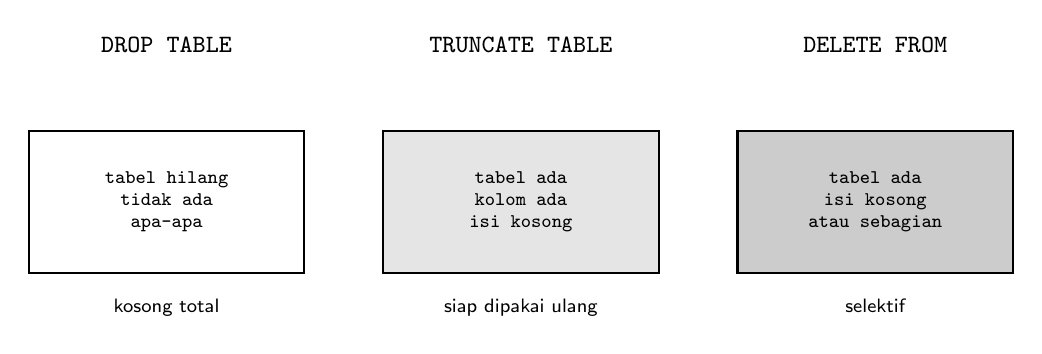
\begin{tikzpicture}[
			tbl/.style={rectangle, draw=black, thick, minimum width=3.5cm, minimum height=1.8cm, align=center, font=\ttfamily\scriptsize},
			title/.style={font=\sffamily\small, align=center}
		]
		\node[title] at (0, 2.5) {\texttt{DROP TABLE}};
		\node[tbl, fill=white] (a) at (0, 0.5) {tabel hilang \\ tidak ada \\ apa-apa};
		\node[font=\scriptsize\sffamily, below=0.2cm of a] {kosong total};

		\node[title] at (4.5, 2.5) {\texttt{TRUNCATE TABLE}};
		\node[tbl, fill=black!10] (b) at (4.5, 0.5) {tabel ada \\ kolom ada \\ isi kosong};
		\node[font=\scriptsize\sffamily, below=0.2cm of b] {siap dipakai ulang};

		\node[title] at (9, 2.5) {\texttt{DELETE FROM}};
		\node[tbl, fill=black!20] (c) at (9, 0.5) {tabel ada \\ isi kosong \\ atau sebagian};
		\node[font=\scriptsize\sffamily, below=0.2cm of c] {selektif};
	\end{tikzpicture}
	\caption{Tiga perintah penghapusan dan hasil akhirnya.}
	\label{fig:drop-vs-truncate}
\end{figure}

Pemilihan ketiganya bergantung pada tujuan. Jika ingin menyingkirkan tabel dari skema, pakai \texttt{DROP}. Jika ingin mengosongkan tabel untuk diisi ulang, pakai \texttt{TRUNCATE}. Jika ingin menghapus sebagian baris atau butuh \texttt{WHERE}, pakai \texttt{DELETE}.

\subsection{Prosedur Aman Sebelum \texttt{DROP TABLE}}

Menghapus tabel dari database produksi adalah salah satu operasi paling berisiko. Gambar~\ref{fig:drop-safe} menyajikan prosedur minimal.

\begin{figure}[H]
	\centering
	\begin{tikzpicture}[
			node distance=0.4cm,
			step/.style={rectangle, draw=black, thick, fill=black!5, text width=9.5cm, align=left, minimum height=0.8cm, font=\sffamily\small, inner sep=8pt},
			line/.style={draw, thick, -latex}
		]
		\node[step] (s1) {\textbf{1.} Periksa foreign key: \texttt{SHOW CREATE TABLE produk\G} dan cari \texttt{REFERENCES}};
		\node[step, below=0.3cm of s1] (s2) {\textbf{2.} Periksa trigger: \texttt{SHOW TRIGGERS LIKE 'produk'}};
		\node[step, below=0.3cm of s2] (s3) {\textbf{3.} Cadangkan: \texttt{mysqldump -u root -p toko\_online produk > produk.sql}};
		\node[step, below=0.3cm of s3] (s4) {\textbf{4.} Verifikasi berkas cadangan: \texttt{ls -lh produk.sql}};
		\node[step, below=0.3cm of s4] (s5) {\textbf{5.} Baru jalankan \texttt{DROP TABLE produk;}};

		\draw[line] (s1) -- (s2);
		\draw[line] (s2) -- (s3);
		\draw[line] (s3) -- (s4);
		\draw[line] (s4) -- (s5);
	\end{tikzpicture}
	\caption{Prosedur aman sebelum \texttt{DROP TABLE}.}
	\label{fig:drop-safe}
\end{figure}

Langkah 1 penting karena \texttt{DROP TABLE} akan gagal jika ada tabel lain yang merujuknya lewat foreign key. Pesan yang muncul seperti berikut.

\begin{lstlisting}[style=out]
ERROR 1217 (23000): Cannot delete or update a parent row:
a foreign key constraint fails
\end{lstlisting}

Untuk mengatasinya, hapus dulu foreign key di tabel anak, atau ubah urutan penghapusan.

\section{Studi Kasus: Evolusi Tabel \texttt{produk}}

Mari ikuti perjalanan sebuah tabel dari lahir, berkembang, sampai pensiun. Setiap perintah disertai keluarannya.

\subsection{Langkah 1: Membuat Tabel Awal}

\begin{lstlisting}[style=code]
CREATE TABLE produk (
    id    INT AUTO_INCREMENT PRIMARY KEY,
    nama  VARCHAR(100) NOT NULL,
    harga DECIMAL(10,2) NOT NULL
);
\end{lstlisting}

\begin{lstlisting}[style=out]
Query OK, 0 rows affected
\end{lstlisting}

\subsection{Langkah 2: Melihat Struktur Awal}

\begin{lstlisting}[style=code]
DESCRIBE produk;
\end{lstlisting}

\begin{lstlisting}[style=out]
+-------+---------------+------+-----+---------+----------------+
| Field | Type          | Null | Key | Default | Extra          |
+-------+---------------+------+-----+---------+----------------+
| id    | int           | NO   | PRI | NULL    | auto_increment |
| nama  | varchar(100)  | NO   |     | NULL    |                |
| harga | decimal(10,2) | NO   |     | NULL    |                |
+-------+---------------+------+-----+---------+----------------+
\end{lstlisting}

\subsection{Langkah 3: Menambah Kolom Stok dan Status}

\begin{lstlisting}[style=code]
ALTER TABLE produk
    ADD COLUMN stok INT UNSIGNED NOT NULL DEFAULT 0,
    ADD COLUMN is_active BOOLEAN NOT NULL DEFAULT TRUE;
\end{lstlisting}

\subsection{Langkah 4: Menambah Kolom SKU di Posisi Khusus}

\begin{lstlisting}[style=code]
ALTER TABLE produk
    ADD COLUMN sku VARCHAR(20) NOT NULL AFTER id;
\end{lstlisting}

\subsection{Langkah 5: Memperpanjang Nama Produk}

\begin{lstlisting}[style=code]
ALTER TABLE produk
    MODIFY COLUMN nama VARCHAR(150) NOT NULL;
\end{lstlisting}

\subsection{Langkah 6: Menambah Indeks pada Harga}

\begin{lstlisting}[style=code]
ALTER TABLE produk
    ADD INDEX idx_harga (harga);
\end{lstlisting}

\subsection{Langkah 7: Memeriksa Seluruh Perubahan}

\begin{lstlisting}[style=code]
SHOW CREATE TABLE produk\G
\end{lstlisting}

Keluaran akan menampilkan \texttt{CREATE TABLE} dengan semua kolom dan indeks yang sudah ditambahkan.

\subsection{Langkah 8: Mengubah Nama Kolom}

\begin{lstlisting}[style=code]
ALTER TABLE produk
    CHANGE COLUMN is_active aktif BOOLEAN NOT NULL DEFAULT TRUE;
\end{lstlisting}

\subsection{Langkah 9: Menghapus Indeks yang Tidak Terpakai}

\begin{lstlisting}[style=code]
ALTER TABLE produk DROP INDEX idx_harga;
\end{lstlisting}

\subsection{Langkah 10: Mengosongkan Isi Tanpa Menghapus Struktur}

\begin{lstlisting}[style=code]
TRUNCATE TABLE produk;
\end{lstlisting}

Setelah \texttt{TRUNCATE}, \texttt{id} yang tadinya \texttt{AUTO\_INCREMENT} akan mulai lagi dari 1.

\subsection{Langkah 11: Menghapus Tabel}

\begin{lstlisting}[style=code]
DROP TABLE produk;
\end{lstlisting}

\subsection{Timeline Studi Kasus}

Gambar~\ref{fig:case-timeline} merangkum sebelas langkah tersebut dalam satu garis waktu.

\begin{figure}[H]
	\centering
	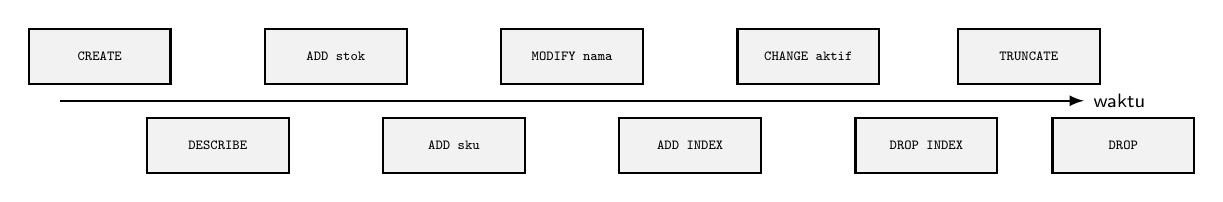
\begin{tikzpicture}[
			ev/.style={rectangle, draw=black, thick, fill=black!5, minimum width=1.8cm, minimum height=0.7cm, font=\ttfamily\tiny, align=center},
			line/.style={draw, thick}
		]
		\draw[line, -latex] (-6, 0) -- (7, 0);
		\node[font=\scriptsize\sffamily, right] at (7, 0) {waktu};

		\node[ev, above=0.2cm] (e1) at (-5.5, 0) {CREATE};
		\node[ev, below=0.2cm] (e2) at (-4, 0) {DESCRIBE};
		\node[ev, above=0.2cm] (e3) at (-2.5, 0) {ADD stok};
		\node[ev, below=0.2cm] (e4) at (-1, 0) {ADD sku};
		\node[ev, above=0.2cm] (e5) at (0.5, 0) {MODIFY nama};
		\node[ev, below=0.2cm] (e6) at (2, 0) {ADD INDEX};
		\node[ev, above=0.2cm] (e7) at (3.5, 0) {CHANGE aktif};
		\node[ev, below=0.2cm] (e8) at (5, 0) {DROP INDEX};
		\node[ev, above=0.2cm] (e9) at (6.3, 0) {TRUNCATE};
		\node[ev, below=0.2cm] (e10) at (7.5, 0) {DROP};
	\end{tikzpicture}
	\caption{Timeline sebelas langkah evolusi tabel \texttt{produk}.}
	\label{fig:case-timeline}
\end{figure}

\section{Kesalahan Umum dan Cara Menghindarinya}

\begin{table}[H]
	\centering
	\caption{Kesalahan umum pada CRUD tabel.}
	\label{tab:mistakes}
	\footnotesize
	\begin{tabularx}{\textwidth}{l X X}
		\toprule
		Kesalahan                                           & Akibat                                   & Perbaikan                                                                     \\
		\midrule
		\texttt{DROP TABLE} tanpa backup                    & kehilangan data permanen                 & \texttt{mysqldump} lebih dulu                                                 \\
		\texttt{TRUNCATE} dikira sama dengan \texttt{DROP}  & tabel masih ada, tetapi isi hilang       & pahami perbedaan pada Tabel~\ref{tab:drop-truncate-delete}                    \\
		\texttt{ALTER TABLE} satu operasi per perintah      & tabel dibangun ulang berkali-kali        & gabungkan beberapa operasi sekaligus                                          \\
		\texttt{MODIFY} dikira bisa ganti nama              & error karena sintaksnya beda             & pakai \texttt{CHANGE} untuk ganti nama                                        \\
		lupa \texttt{FIRST} atau \texttt{AFTER}             & kolom baru selalu di akhir               & tambahkan posisi jika perlu                                                   \\
		\texttt{ADD INDEX} untuk kolom yang jarang difilter & indeks tidak terpakai, hanya makan ruang & indeks hanya untuk kolom yang sering di \texttt{WHERE} atau \texttt{ORDER BY} \\
		\texttt{DROP COLUMN} tanpa cek foreign key          & error karena ada referensi               & cek \texttt{SHOW CREATE TABLE} tabel anak                                     \\
		mengira \texttt{SHOW TABLES} menampilkan isi        & hanya nama tabel                         & pakai \texttt{SELECT} untuk isi                                               \\
		\texttt{CREATE TABLE} tanpa primary key             & sulit melakukan update selektif          & selalu sediakan primary key                                                   \\
		\texttt{AUTO\_INCREMENT} untuk ID publik            & ID mudah ditebak, rawan scraping         & \texttt{UUID\_SHORT()} atau \texttt{BINARY(16)}                               \\
		\bottomrule
	\end{tabularx}
\end{table}

\section{Lembar Rujukan Cepat}

\begin{table}[H]
	\centering
	\caption{Rujukan cepat perintah CRUD pada tingkat tabel.}
	\label{tab:cheat}
	\footnotesize
	\begin{tabularx}{\textwidth}{l l X}
		\toprule
		Operasi & Perintah                                            & Keterangan              \\
		\midrule
		Create  & \texttt{CREATE TABLE nama (...)}                    & tabel baru              \\
		Create  & \texttt{CREATE TABLE IF NOT EXISTS}                 & aman untuk skrip        \\
		Create  & \texttt{CREATE TABLE baru LIKE lama}                & salin struktur          \\
		Create  & \texttt{CREATE TABLE baru AS SELECT}                & salin struktur dan data \\
		Read    & \texttt{SHOW TABLES}                                & daftar tabel            \\
		Read    & \texttt{DESCRIBE nama}                              & ringkasan kolom         \\
		Read    & \texttt{SHOW CREATE TABLE nama\G}                   & definisi lengkap        \\
		Read    & \texttt{SHOW INDEX FROM nama}                       & daftar indeks           \\
		Read    & \texttt{SELECT * FROM information\_schema.tables}   & query katalog           \\
		Update  & \texttt{ALTER TABLE ADD COLUMN}                     & tambah kolom            \\
		Update  & \texttt{ALTER TABLE DROP COLUMN}                    & hapus kolom             \\
		Update  & \texttt{ALTER TABLE MODIFY COLUMN}                  & ubah definisi           \\
		Update  & \texttt{ALTER TABLE CHANGE COLUMN}                  & ubah nama dan definisi  \\
		Update  & \texttt{ALTER TABLE RENAME TO}                      & ganti nama tabel        \\
		Update  & \texttt{ALTER TABLE ADD INDEX}                      & tambah indeks           \\
		Update  & \texttt{ALTER TABLE DROP INDEX}                     & hapus indeks            \\
		Update  & \texttt{ALTER TABLE ADD PRIMARY KEY}                & tambah primary key      \\
		Update  & \texttt{ALTER TABLE ADD CONSTRAINT ... FOREIGN KEY} & tambah foreign key      \\
		Delete  & \texttt{DROP TABLE [IF EXISTS] nama}                & hapus tabel             \\
		Delete  & \texttt{TRUNCATE TABLE nama}                        & kosongkan isi           \\
		\bottomrule
	\end{tabularx}
\end{table}

\section{Kesimpulan}

CRUD pada tingkat tabel adalah wilayah dengan permukaan terluas di seluruh basis data relasional. Dari satu perintah \texttt{CREATE} hingga dua belas varian \texttt{ALTER}, semuanya bermuara pada satu prinsip: struktur tabel adalah kontrak yang bisa berubah, tetapi setiap perubahan punya biaya. Tiga prinsip penutup:

\begin{enumerate}
	\item Create dengan niat. Setiap kolom punya alasan; setiap tipe punya konsekuensi; setiap \texttt{DEFAULT} menghemat satu baris di \texttt{INSERT}. Selalu sediakan primary key, dan pilih \texttt{IF NOT EXISTS} untuk skrip yang akan dijalankan berulang.
	\item Read sebagai kebiasaan. \texttt{DESCRIBE} untuk melihat cepat, \texttt{SHOW CREATE TABLE} untuk verifikasi menyeluruh, dan \texttt{information\_schema} untuk otomatisasi. Ketiganya lebih cepat daripada menebak.
	\item Update dan Delete dengan sadar. Gabungkan beberapa \texttt{ALTER} dalam satu perintah untuk tabel besar. Bedakan \texttt{DROP}, \texttt{TRUNCATE}, dan \texttt{DELETE} sesuai tujuan. Selalu backup sebelum \texttt{DROP}.
\end{enumerate}

Dengan fondasi ini, pembaca siap melangkah ke CRUD tingkat baris, di mana \texttt{INSERT}, \texttt{SELECT}, \texttt{UPDATE}, dan \texttt{DELETE} akan menjadi fokus.

\newpage
\section*{Referensi}
\addcontentsline{toc}{section}{Referensi}

\begin{thebibliography}{99}
	\bibitem{mariadb-ddl} MariaDB Foundation. (2026). \textit{SQL Statements --- CREATE TABLE, ALTER TABLE, DROP TABLE, TRUNCATE TABLE, SHOW TABLES, DESCRIBE}. MariaDB Knowledge Base. \texttt{https://mariadb.com/kb/en/sql-statements/}.
	\bibitem{mysql-ddl} Oracle Corporation. (2026). \textit{MySQL 8.0 Reference Manual --- Data Definition Statements}. \texttt{https://dev.mysql.com/doc/refman/8.0/en/sql-data-definition-statements.html}.
	\bibitem{mysql-information-schema} Oracle Corporation. (2026). \textit{MySQL 8.0 Reference Manual --- INFORMATION\_SCHEMA Tables}. \texttt{https://dev.mysql.com/doc/refman/8.0/en/information-schema.html}.
	\bibitem{postgresql} The PostgreSQL Global Development Group. (2026). \textit{SQL Commands --- CREATE TABLE, ALTER TABLE, DROP TABLE, TRUNCATE}. \texttt{https://www.postgresql.org/docs/current/sql-commands.html}.
	\bibitem{silberschatz} Silberschatz, A., Korth, H. F., \& Sudarshan, S. (2019). \textit{Database System Concepts} (7th ed.). McGraw-Hill Education.
	\bibitem{date} Date, C. J. (2003). \textit{An Introduction to Database Systems} (8th ed.). Addison-Wesley.
	\bibitem{kleppmann} Kleppmann, M. (2017). \textit{Designing Data-Intensive Applications}. O'Reilly Media.
	\bibitem{innodb} Oracle Corporation. (2026). \textit{MySQL 8.0 Reference Manual --- InnoDB Storage Engine}. \texttt{https://dev.mysql.com/doc/refman/8.0/en/innodb-storage-engine.html}.
	\bibitem{mysqldump} MariaDB Foundation. (2026). \textit{mariadb-dump}. MariaDB Knowledge Base. \texttt{https://mariadb.com/kb/en/mariadb-dump/}.
	\bibitem{rfc4122} Leach, P., Mealling, M., \& Salz, R. (2005). \textit{A Universally Unique IDentifier (UUID) URN Namespace} (RFC 4122). IETF.
\end{thebibliography}

\end{document}
